\section{Introduction} \label{toc:einleitung}

\subsection{Motivation and Introduction} \label{toc:motivation}

The principle of a software-based and decentralized financial system was first described in 2008 with the cryptocurrency \ac{BTC}.\footcite[Cf.][]{nakamoto2008bitcoin}
The basic principle is the provision of a decentralized ledger,
which records all transactions between participants.\footcite[Cf.][]{badertscher2017bitcoin} In order to verify these transactions,
the principle of "mining" was introduced. By making computing power available, the decentralized 
network and thereby secure transactions in the blockchain.\footcite[Cf.][]{kroll2013economics} The voluntary provision of
of computing power is rewarded with the payment of Bitcoins to the owner of the hardware. Initially, it paid out to do Bitcoin
Mining in a private environment with comparatively weak hardware. As interest in Bitcoin increased, so did the number of
of individuals and groups engaged in mining. Due to the resulting increase in the overall computing power of the network, at a certain point
private mining ceased to be profitable, since the maintenance and operating costs of the hardware
exceeded the mining revenue. Subsequently, the business case of "cloud mining" has emerged.\footcite[Cf.][]{taylor2017evolution} This describes
providers that operate data centers specifically for mining cryptocurrencies and sell this service to customers on a pro-rata basis,
who can profit depending on their share of bitcoin payouts from mining.\footcite[Cf.][chap. 3.4.5]{bhaskar2015bitcoin}
To have the profit margin as large as possible for the operating company, there are many factors to consider when building and operating
such data center. The profit margin in operation is basically the difference between the revenue generated by mining
and on the other hand the operating costs and customer payouts. The revenue can be increased by optimizing the efficiency of the hardware.
Operating expenses are largely determined by electricity, spare parts and personnel costs. All these cost items
can be optimized by suitable tools. In addition, after a certain period of time, the start-up investment, such as land, real estate and hardware
must be amortized so that the company is able to make a profit. In such a company (Genesis Group),
which offers cloud mining and owns data centers worldwide, the following thesis takes place. 

One way to visualize and optimize the revenues and expenses of such data centers is to introduce a 
\ac{BI} process. Such are already used to optimize financial data, among other things.\footcite[Cf.][pp. 105]{azma2012business} 
In a \ac{BI} process, data is collected in the first step, subsequently analyzed, and presented to stakeholders at the end,
in order to make decision-making processes transparent and to simplify them.\footcite[Cf.][pp. 1]{loshin2012business} 
In-house data is already collected from \ac{ERP} systems and mining hardware monitoring. 
However, this data is not used further and therefore not submitted to analysis. The analysis and calculation of financial data is
currently supported by a Monte Carlo simulation. However, only idealized data from the data centers are used as starting parameters and 
no real data from the survey are used, since these are not available at this time. In addition, the input parameters are
only estimated. All these components should be combined for a meaningful extension of a \ac{BI} process. The stakeholders of
such a process in this case are the top management and the controlling department, which can use
real data to get a much improved financial picture of a data center. Whether this is reasonably possible 
and how such an implementation can look like, will be clarified in the following of this thesis. The aim is to improve the financially relevant data of a data 
data center and thus to be able to optimize it. 

\subsection{Hypotheses and delimitation of the thesis} \label{toc:hypothesenundabgrenzungderarbeit}

After the thorough analysis of the subject area \ac{BI} and the internal company requirements, the following main hypothesis was 
formulated: 

\textbf{\ac{HT0}: }By introducing a business intelligence process, it is possible to optimize the profitability of a cryptomining
data center. 

In order to be able to work on the main hypothesis better, several sub-hypotheses are formed from this, which divides the main hypothesis into
meaningful subareas. This process has resulted in four sub-hypotheses, which are formulated as follows: 

\textbf{\ac{HT0.1}: }A business intelligence process is used to help management make decisions regarding the
new construction and expansion of mining data centers. 

\textbf{\ac{HT0.2}: }Existing hardware in mining data centers will be optimized by implementing business intelligence. 

\textbf{\ac{HT0.3}: }Business intelligence will improve cash flow evaluation at a mining data center. 

\textbf{\ac{HT0.4}: }Staff planning for a mining data center is optimized through business intelligence processes. 

\ac{HT0.1} deals with the new construction and expansion of data centers. The three other sub-hypotheses are relevant during the operation of a
Cryptomining data center relevant. In the following, all sub-hypotheses are outlined: 

\begin{itemize} 
    \item \textbf{\ac{HT0.1}: }The expansion and new construction of mining data centers is essential for the further development of cloud mining,
    as this will increase the revenue generated by mining. In this context, many influencing factors, such as intrinsic mining
    parameters (Cf. chap. \ref{toc:miningundkonsensalgorithmen}), price developments in the \ac{BTC} market, financial drivers, and \acp{KPI}
    (Cf. chap. \ref{toc:kennzahlenundeinflussfaktoren}) of a data center should be taken into account. Due to the complexity and amount of
    different data, \ac{BI} could be a way to support this important strategic process. 
    \item \textbf{\ac{HT0.2}: }The second sub-hypothesis is limited to the technical factors that can contribute to increasing the efficiency of the
    Mining process can contribute. Here, the technical parameters of the hardware are used to identify possible points for improvement
    to identify. This refers to the basics of mining described in chapter \ref{toc:miningundkonsensalgorithmen}.
    By applying a \ac{BI} process to the technical parameters, an attempt is made to optimize the efficiency of the existing hardware in this area..
    \item \textbf{\ac{HT0.3}: }In this sub-hypothesis, financial \acp{KPI} are considered. In chapter
    \ref{toc:kennzahlenundeinflussfaktoren}, these are identified for a mining data center. This hypothesis uses the financial
    metrics and \acp{KPI} that are made visible by implementing a \ac{BI} Process. This allows optimization potentials to be
    found that would be difficult to see without \ac{BI}. The financial optimization ultimately improves the cash flow of a
    data center. 
    \item \textbf{\ac{HT0.4}: }The last sub-hypothesis addresses workforce planning. In a data center, personnel costs are incurred by
    hiring maintenance and local management staff. By analyzing the work involved, such as the
    repair of equipment defects, the staff scheduling of a mining data center can be optimized. This analysis is to be performed by means of a
    \ac{BI} process.
\end{itemize}


All four sub-hypotheses cover the entire spectrum of the main hypothesis with their respective perspectives (technology, finance, personnel, new construction and expansion).

In the following work, some limitations are made. Care is taken to ensure that this does not falsify the research result 
and that the delimitation makes the argumentation more transparent and comprehensible. The following delimitations are made: 

\begin{itemize} 
    \item Only the cryptocurrency Bitcoin is considered. 
    \item As a result, only Bitcoin's \ac{PoW} consensus algorithm is used as the basis for the research. 
    \item There are a variety of different specialized mining hardware on the market. The performance of this hardware is measured by identical 
    parameters. Therefore, one mining hardware model (Antminer S19Pro) is used as an example for the analyses in this work. 
    \item A concrete technical elaboration of a \ac{BI} process as well as its underlying systems is omitted. The focus of this
    focus on the perspective of a \ac{BI} stakeholder and the project management. 
    \item There will be no quantitative or empirical analysis of the hypothesis. The work will rely on qualitative and argumentative 
    deductive analysis as well as a case study.
\end{itemize}

\subsection{Design and structure of the thesis} \label{toc:aufbauundstruktur}

The formulation of the main hypothesis results in the theoretical foundations which have to be treated in depth for the answer.
This is in the first step the analysis of \ac{BI} Processes and their fundamentals. In chapter \ref{toc:grundlagenbusinessintelligence}
the basic characteristics of \ac{BI}, their operational added value and the prerequisites that a company must fulfill are analyzed.
The next step is to lay the foundations for understanding mining and cryptomining data centers. To achieve this,
in chapter \ref{toc:grundlagenkryptomining} is outlined, how blockchains and the mining of cryptocurrencies work. Building on this
a mining data center will be analyzed exemplarily, where in the first step the structure and the functionality and following the central
financial drivers and \acp{KPI} are analyzed. In chapter \ref{toc:ansatzmoeglichkeitenfuerbusinessintelligence} the two
basic parts are used to identify starting points for the introduction of a \ac{BI} process will be identified. In the process, the testing of the
hypotheses is carried out. In the last chapter of the main part, a concrete implementation and modeling of a \ac{BI} Process
is elaborated. Thus, by means of a case study, it is verified whether the elaborated principles from chapter
\ref{toc:ansatzmoeglichkeitenfuerbusinessintelligence} can be implemented in reality and whether the answers to the hypotheses are robust.
Finally, the conclusion critically examines this work and identifies possible starting points for further research.
are identified.

\subsection{Relevance in business informatics} \label{toc:relevanzinderwirtschaftinformatik}

Information systems is an interdisciplinary science that is composed of economics and computer science.\footcite[Cf.][p. 5]{mertens2005grundzuge}
One of the long-term goals of business informatics is the meaningful
automation of processes.\footcite[Cf.][p. 4]{mertens2005grundzuge} This means that tasks are transferred from humans to application systems,
where this makes sense from a business point of view.\footcite[Cf.][p. 4]{mertens2005grundzuge}
Business intelligence is an approach that involves both economic and technical aspects and is therefore directly
in the area of business informatics.\footcite[Cf.][p. 102]{azma2012business} The economic part is primarily to be found in the area of business processes.
The technical part extends toward Big Data and business analytics. "The
team needs a champion [...] who understands the business and the technology and is able to translate the business requirements into a
(high-level) \ac{BI} architecture for a system."\footcite[][p. 27]{yeoh2010critical} This is precisely the kind of task for which business informatics
is of central importance.

The field of cryptocurrencies is characterized by both technical and economic approaches, and thus should be viewed in the business informatics
to be viewed in order to be able to adequately appreciate both sub-aspects.\footcite[Cf.][]{derks2018chaining} In this work, we examine,
whether it is possible to use business intelligence to optimize the mining of cryptocurrencies in a data center environment.
For the reasons stated above, this work falls within the domain of business intelligence. The relevance for
business informatics results from the combination of the two topics (business intelligence and cryptomining) in order to achieve a
financial optimization. It is indispensable to analyze and classify technical as well as business aspects in order to
and to classify, in order to be able to examine and finally verify the hypotheses of the work.

\subsection{Methodology and source selection} \label{toc:methodikundquellenauswahl}

In order to make the testing of the hypotheses robust, this part explains the methodology used, on which this work is based.
Furthermore, the selection and research process for the literature used is the subject of this chapter. 

At the beginning of the conception of this thesis, the literature research and thereby an identification of the research gap, which is to be closed with this thesis, was carried out.
The research follows the principles suggested by Brocke et al.\footcite[Cf.][]{brocke2009reconstructing}
It should be noted that the procedure will not be carried out in the full depth suggested by Brocke et al. as the
focus of this paper is not on the systematic search of literature and a literature review. Therefore, the process of the search is described in the following. 

\begin{figure}[H] 
    \caption{Procedure in the literature search process} 
    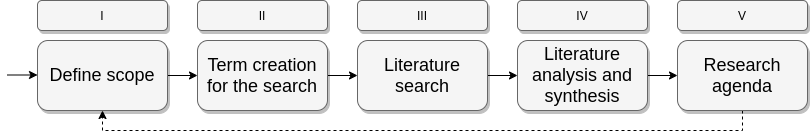
\includegraphics[width=0.9\textwidth]{literaturereview} 
    \label{figure:literaturereview} 
    \\ 
    \cite[Source: Based on][Fig. 3]{brocke2009reconstructing} 
\end{figure} 

The research is divided into a five-step process that is worked through sequentially
(Cf. Fig. \ref{figure:literaturereview}):\footcite[Cf.][pp. 2211]{brocke2009reconstructing} 

\begin{enumerate} 
    \item The first step is to define the scope of the literature review. In this case, this was done on the basis of the topics \ac{BI} and
    the mining of cryptocurrencies. In table \ref{tbl:literaturtaxonomie} the result for the first step is shown. In
    this table, a literature taxonomy is performed according to Cooper.\footcite[Cf.][p. 2212]{brocke2009reconstructing}\footcite[Cf.][]{cooper1988organizing} 
    \item Following, the search terms for the literature search are formed. However, this step is continuously adapted depending on
    the results. Abbreviations as well as German and English terms are searched for. The used 
    search queries are listed in table \ref{tbl:suchprozessergebnis}.\footcite[Cf.][pp. 2211]{brocke2009reconstructing} 
    \item In this step, the actual literature is searched. The search platforms used are Google
    Scholar\footnote{https://scholar.google.com}, EBSCO\footnote{https://www.ebsco.com}, Wiso\footnote{https://www.wiso-net.de}, 
    SpringerLink\footnote{https://link.springer.com}, and IEEExplore\footnote{https://ieeexplore.ieee.org}. Care is taken to
    that, whenever possible, these are peer-reviewed publications that have appeared in scientific journals.
    Books and online sources are also used to some extent. However these are not used as a basis for the central
    argumentation of the paper, as these books cannot be considered scientific literature. The result of the
    search can be found in table \ref{tbl:suchprozessergebnis}. 
    \item Now the literature is analyzed and structured. For this purpose, subject areas are defined, to which the found literature is assigned
    to. The result of this can be found in table \ref{tbl:konzeptmatrix}.\footcite[Cf.][p. 2214]{brocke2009reconstructing}\footcite[Cf.][]{webster2002analyzing}  
    \item The final step is to develop the research agenda based on the research gap. This is in this work in
    the application of \ac{BI} in the field of mining cryptocurrencies. There are numerous publications on the optimization of mining
    processes.\footcite[Cf.][]{han2019demystifying}\footcite[Cf.][]{courtois2014optimizing} In addition, there are publications in the
    area of mining hardware as well as mining and blockchains in the cloud.\footcite[Cf.][]{taylor2017evolution}\footcite[Cf.][]{gai2020blockchain} 
    Furthermore, research papers can be found in the area of building mining data centers. These tend to focus on the construction of
    \ac{ASIC} based data centers, which is appropriate for Bitcoin.\footcite[Cf.][]{li2019blockchain}\footcite[Cf.][]{xie2018extreme}
    The data centers under consideration operate mining exclusively through \ac{ASIC} based hardware. Accordingly, there are numerous publications on the
    Cryptomining side and on the topic of mining optimization. When looking for a connection between
    cryptomining and \ac{BI}, however, the selection is much smaller. There is literature that deals with the combination of
    cryptocurrencies and \ac{BI}, but this tends to be in the area of rates and rate trends.
    is.\footcite[Cf.][]{botocs2017bitcoin} Nothing can be found in the area of optimizing mining infrastructures using \ac{BI}.
    On the one hand, this is due to a few large companies that operate bitcoin mining and that do not publish their optimizations and efficiencies
    due to the fierce competition.\footcite[Cf.][]{btccom2021miner} On the other hand, the cryptocurrency hype of the
    last few years is more in the area of investing and advancing blockchain technology and less in the area of
    Mining.\footcite[Cf.][]{friedlmaier2018disrupting} 
\end{enumerate}

\begin{figure}[H]
    \caption{Method profile of business informatics}
    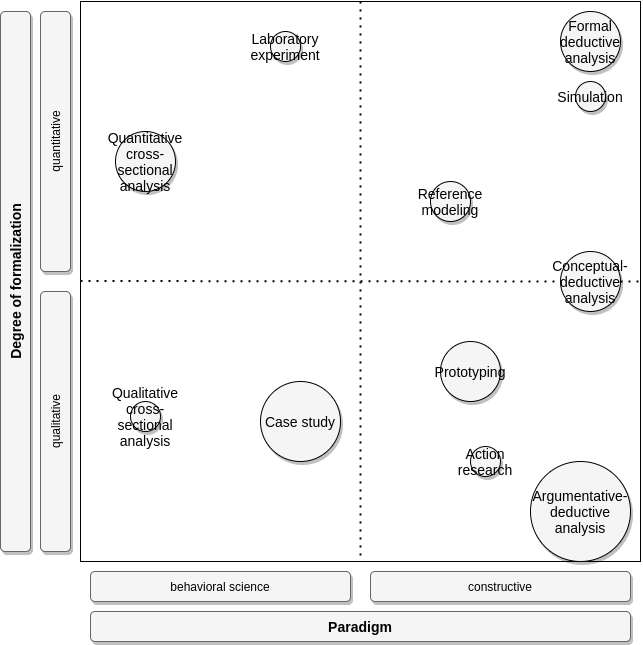
\includegraphics[width=0.7\textwidth]{methodenprofilwi}
    \label{figure:methodenprofilwi}
    \\
    \cite[Source: Based on][Fig. 3]{wilde2007forschungsmethoden}
\end{figure}

For the evaluation of the right methodology to test the hypotheses of this thesis, the possible methodologies in
information systems in general and in the field of \ac{BI} in particular
are analyzed.\footcite[Cf.][]{wilde2007forschungsmethoden}\footcite[Cf.][]{wilde2006methodenspektrum}\footcite[Cf.][]{jourdan2008business} 
It can be noted that both argumentative-deductive analysis and case study occupy the first two places in terms of
use.\footcite[Cf.][Fig. 2]{wilde2007forschungsmethoden} Also, in the majority of publications in the field of
\ac{BI} use qualitative methods.

To be able to test the hypotheses the following qualitative methodologies are used:

\begin{itemize}
    \item \textbf{argumentative-deductive analysis: }This is a construction science method that is built primarily on the
    the application of a logical chain of reasoning.\footcite[Cf.][Tbl. 1]{wilde2007forschungsmethoden} This is discussed in chapter
    \ref{toc:ansatzmoeglichkeitenfuerbusinessintelligence} and is based on the foundations of the previous two chapters.
    An argumentative-deductive analysis is used to conduct the first test of the hypotheses. 
    \item \textbf{case study: }In chapter \ref{toc:planungeinesbiprozessesfuereinminingrechenzentrum} a case study is designed based on the theoretical
    results, a case study will be designed. This will be qualitative in nature and will represent a further test of the hypotheses. In
    difference to the argumentative-deductive analysis, the case study will test the hypotheses in a real environment.
    Therefore, a case study does not belong to the construction science methods, but to the behavioral science methods
    (Cf. Fig. \ref{figure:methodenprofilwi}). In designing the case study, we will follow the publication of Göthlich\footcite[Cf.][]{gothlich2003fallstudien}
    The stakeholder analysis is based on the publication of Simmers
    is undertaken.\footcite[Cf.][]{simmers2004stakeholder} The analysis of an introduction is primarily examined through the texts of Loshin and
    Boyer et al. reviewed.\footcite[Cf.][]{loshin2012business}\footcite[Cf.][]{boyer2010business}
\end{itemize} 

By testing the hypotheses using two independent methodologies, an attempt is made to ensure that the hypotheses are analyzed from different points of view
and thus the result of this work is resilient.
